\section{Respostas das Questões do Protocolo}

Nesta seção são respondidas as questões definidas no Protocolo de MSL, apresentado no início deste capítulo, levando em consideração a análise dos resultados da seção anterior.
Assim, seguem:

\begin{enumerate}
      \item Quais são as principais soluções de acessibilidade para PDV utilizadas
            no desenvolvimento de aplicações móveis?
            \begin{enumerate}
                  \item Foi observado o cumprimento de diretrizes de acessibilidade para aplicações móveis propostas por entidades
                        como Google\footnote{\url{https://developer.android.com/guide/topics/ui/accessibility/apps}},
                        SIDI\footnote{\url{https://www.sidi.org.br/guiadeacessibilidade}} e
                        BBC\footnote{\url{https://www.bbc.co.uk/accessibility/forproducts/guides/mobile}}; não foi identificado, porém, o uso das diretrizes da
                        Apple\footnote{\url{https://developer.apple.com/design/human-interface-guidelines/accessibility/overview/introduction/}};
                  \item Realização de estudos visando identificar problemas enfrentados por usuários com DV no uso de aplicativos móveis e definir diretrizes para solucionar cada problema;
                  \item Utilização de diretrizes de acessibilidade da W3C\footnote{\url{https://www.w3.org/TR/mobile-bp/summary}} adaptadas da \emph{web} para o contexto de aplicações móveis;
                  \item Utilização de ferramentas para realização de testes de acessibilidade automatizados.
            \end{enumerate}
      \item Quais são as tecnologias utilizadas no desenvolvimento dessas soluções?
            \begin{enumerate}
                  \item A linguagem Java no desenvolvimento de aplicações Android;
                  \item Os \emph{frameworks} React Native, Cordova e MD² no desenvolvimento multiplataforma;
                  \item As IDEs Android Studio e Eclipse;
                  \item Unity 3D no desenvolvimento de jogos para Android;
                  \item As ferramentas Accessibility Scanner App, MATE e Test Lab para realização de testes de acessibilidade automatizados.
            \end{enumerate}
      \item Para quais plataformas as soluções foram propostas?
            \begin{enumerate}
                  \item 9 apenas para Android;
                  \item 2 apenas para iOS\@;
                  \item 4 multiplataforma, para Android e iOS\@.
            \end{enumerate}
      \item Quem são os públicos alvos dessas soluções? \\
            As soluções visaram atender diversas necessidades de PDV\@.
            Assim, foram criadas aplicações para diferentes públicos com DV,
            como crianças e estudantes, e com diversos tópicos específicos,
            como livros, medicamentos e clima.
\end{enumerate}

\section{Técnicas Propostas para o DiaVision}

A \autoref{tab_tec_pro} relaciona as técnicas para solução de problemas de acessibilidade à DV, listadas na \autoref{tab-tec-uti-des-1},
utilizadas no desenvolvimento das aplicações nos estudos do MSL, com as propostas para implementação no aplicativo
desenvolvido no presente trabalho, o DiaVision.
\begin{table}
      \caption{Relação de técnicas adotadas pelos artigos e propostas para o DiaVision.}
      \label{tab_tec_pro}
      \begin{center}
            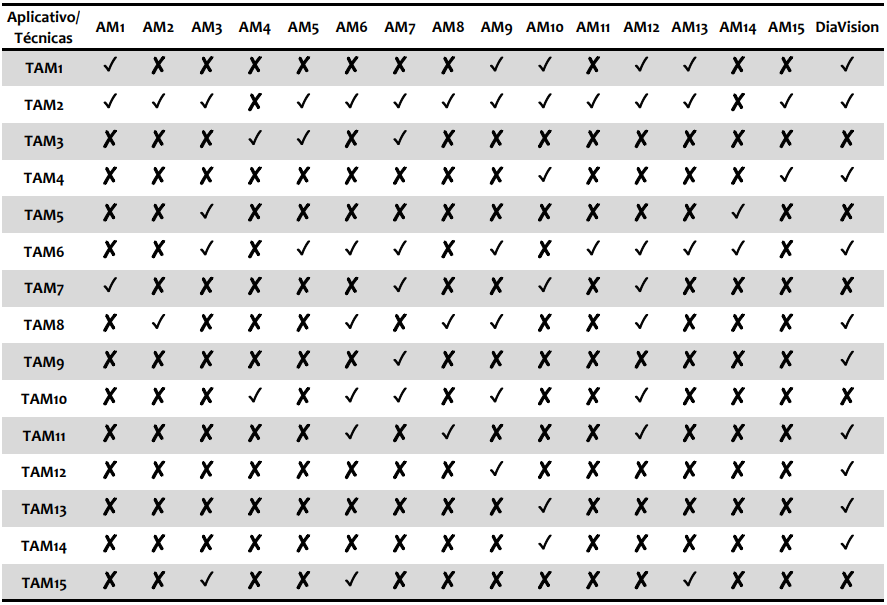
\includegraphics[scale=0.68]{Imagens/proposta/tecnicas_propostas.png}
      \end{center}
      \legend{Fonte: Autor.}
\end{table}

\section{Considerações Finais}

Este capítulo buscou realizar um levantamento, por meio de um estudo de MSL, do estado da arte
acerca dos problemas de acessibilidade enfrentados por PDV e das soluções para os mesmos.
A partir da análise dos resultados, ficou evidente a necessidade de preocupação com
acessibilidade no processo desenvolvimento de soluções para dispositivos móveis.
Sendo identificadas 15 das principais soluções para resolver diferentes problemas relacionados à DV,
das quais 10 foram consideradas no desenvolvimento da solução proposta,
que será descrita no próximo capítulo.